Energię potencjalną będącą wynikiem oddziaływania kulombowskiego pomiędzy pojedynczym elektronem i protonem w atomie wodoru opisuje poniższy wzór:\newline
$ U(r) = \dfrac{e^2}{4\pi \epsilon_0 r} $, gdzie:\newline
$ r $ - odległość elektronu od protonu.\newline
Energia potencjalna jest funkcją odległości r od jądra. Jest to pole centralne.

\begin{figure} [H]
	\centering
	\begin{subfigure}{.99\textwidth}
		\centering
		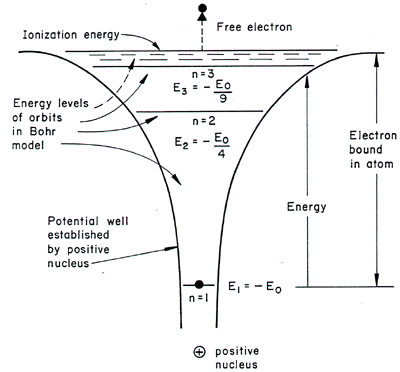
\includegraphics[width=1.0\linewidth]{generalIssues/Figures/potential.png}
	\end{subfigure}
	\caption{Energia potencjalna oddziaływania kulombowskiego pomiędzy elektronem, a jądrem w atomie wodoru.}
	\label{maxwell}
\end{figure}

Równanie Schrodingera dla takiego potencjału ma postać:\newline
$ -\dfrac{\hbar}{2m_e} \nabla^2 \Psi(\vec{r}) = (E-U(\vec{r})) \Psi(\vec{r}) $\newline

Równanie to można rozwiązać przechodząc do układu współrzędnych sferycznych, a następnie sprowadzając je do układu równań jednowymiarowych stosując separację zmiennych:\newline
$ \Psi(\vec{r}) = R(r)\Theta(\theta)\phi(\varphi) $\newline
Rozwiązanie dla funkcji $ \phi(\varphi) $:\newline
$ \phi(\varphi) = e^{im_l \varphi} $ implikuje:\newline
$ e^{im_l 0} = e^{im_l 2\pi} $, warunek ten jest spełniony gdy:\newline
$ |m_l| = 0, 1, 2, 3 ... $.

Liczba kwantowa $ m_l $, nazywana magnetyczną liczbą kwantową,jest związana z orientacją w przestrzeni wektora momentu pędu. Jeżeli atom znajduje się w zewnętrznym polu magnetycznym, to jego energia zależy od tej liczby kwantowej. Liczba kwantowa $ m_l $ może być tylko liczbą całkowitą. 

Rozwiązanie dla funkcji $ \Theta(\theta) $ implikuje istnienie liczby kwantowej $ l = |m_l|, |m_l|+1, |m_l|+2 ... $ nazywanej orbitalną liczbą kwantową, będącą miarą wielkości momentu pędu związanego ze stanem kwantowym: \newline
$ L = \hbar \sqrt{l(l+1)} $ - orbitralny moment pędu.\newline
$ L_z = \hbar m_l $ - rzut wektora momentu pęduna oś OZ.\newline
Obie powyższe wielkości są skwantowane.

Dostępne stany energii opisuje równanie:\newline
$ E = -\dfrac{1}{2} m_e c^2 (Z\alpha)^2 \dfrac{1}{n_r + l + 1} $, gdzie:\newline
$ Z $ - liczba atomowa (dla wodoru $ Z $ = 1),\newline
$ \alpha \approx 1/137 $ - stała struktury subtelnej,\newline
$ n_l = 0, 1, 2 ... $ - radialna liczba kwantowa,\newline
$ n = n_r + l + 1 $ - główna liczba kwantowa (jest zawsze całkowitą liczbą dodatnią).

Jest to dokładnie ten sam wzór, który wynika z modelu Bohra dla energii dozwolonych stanów związanych.

Np. dla energii $ E_0 = E(n = 1) $ mamy tylko jeden możliwy stan ($n = 1, l = 0, m_l = 0$). Energii $ E_1 = E(n = 2) $ odpowiadają cztery zdegenerowane stany:\newline
($n = 2, l = 0, m_l = 0$),\newline
($n = 2, l = 1, m_l = +1$),\newline
($n = 2, l = 1, m_l = 0$),\newline
($n = 2, l = 1, m_l = -1$).